\section{Functions}

\begin{frame}{Python Functions}
    \begin{itemize}
        \item \textbf{Reusable Code Blocks:} Functions encapsulate blocks of code for repeated use.
        \item \textbf{Modularity:} They break down large programs into smaller, manageable parts.
        \item \textbf{Abstraction:} Functions hide implementation details, focusing on what they do.
        \item \textbf{Inputs and Outputs:}
            \begin{itemize}
                \item Functions can accept \textbf{parameters} (inputs).
                \item They can return \textbf{values} (outputs) using the \texttt{return} statement.
            \end{itemize}
        \item \textbf{Definition:}
            \begin{itemize}
                \item Defined using the \texttt{def} keyword.
                \item Indented code block follows the function definition.
            \end{itemize}
        \item \textbf{Benefits:}
            \begin{itemize}
                \item Code reusability.
                \item Improved readability.
                \item Better organization.
                \item Easier debugging.
            \end{itemize}
    \end{itemize}
    
    \end{frame}



\begin{frame}
    \frametitle{Functions}
\begin{itemize}
    \item \textbf{Function} is a block of code that performs a specific task.
    \item \textbf{Function Declaration} is a statement that defines a function.
    \item \textbf{Function Call} is a statement that executes a function.
    \item \textbf{Function Definition} is a statement that defines the code that the function executes.
    \item \textbf{Function Prototype} is a statement that declares the function's name, return type, and parameters.
    \item \textbf{Function Parameters} are variables that are passed to a function.
\end{itemize}
\end{frame}
    
\begin{frame}
    \frametitle{Functions}
    \begin{itemize}
    \item \textbf{Function Arguments} are values that are passed to a function.
    \item \textbf{Return Type} is the data type of the value that a function returns.
    \item \textbf{Return Statement} is a statement that returns a value from a function.
    \item \textbf{Void Function} is a function that does not return a value.
    \item \textbf{Value-Returning Function} is a function that returns a value.
    \item \textbf{Function Overloading} is the ability to define multiple functions with the same name but different parameters.
    \item \textbf{Function Recursion} is the ability of a function to call itself.
    \end{itemize}
\end{frame}

% \begin{frame}[fragile]
%     \frametitle{Function Definition}
%     \lstinputlisting[style=colorful, language=Python]{/Users/nithinvadekkapat/work/alg-ds/scripts/square-root.py}
% \end{frame}

\begin{frame}{Key Concepts: Scope}
    \begin{itemize}
      \item Local scope: Variables defined within a function.
      \item Enclosing scope: The scope of the outer function containing the inner function.
      \item Global scope: Variables defined outside any function.
    \end{itemize}
  \end{frame}

\begin{frame}{Introduction to Scoping}
    \begin{itemize}
      \item Scoping determines how variables are accessed.
      \item It's like rules for finding the "right box" (variable).
      \item Two main types: Static and Dynamic.
    \end{itemize}
  \end{frame}
  
  \begin{frame}[fragile]{Static Scoping (Python)}
    \begin{itemize}
      \item Scope determined by code structure (lexical).
      \item Determined at compile time.
    \end{itemize}
    \begin{lstlisting}[language=Python]
  x = 10
  def outer():
      x = 20
      def inner():
          print("Inside Inner (Python):", x)
      inner()
      standalone()
  
  def standalone():
      print("Inside Standalone (Python):", x)
  
  outer()
  standalone()
    \end{lstlisting}
  \end{frame}


  \begin{frame}[fragile]{Dynamic Scoping (Bash)}
    \begin{itemize}
      \item Scope determined by call stack (runtime).
      \item Depends on the calling sequence.
    \end{itemize}
    \begin{lstlisting}[language=bash]
  #!/bin/bash
  x=10
  function outer {
    local x=20
    inner
    standalone
  }
  function inner {
    echo "Inside Inner (Bash): $x"
  }
  function standalone {
    echo "Inside Standalone (Bash): $x"
  }
  outer
    \end{lstlisting}
  \end{frame}

  \begin{frame}{Key Differences}
    \begin{itemize}
      \item \textbf{Python (Static):} Definition location matters.
      \item \textbf{Bash (Dynamic):} Call location matters.
      \item Static: Predictable, easier to debug.
      \item Dynamic: Runtime customizations, but harder to reason about.
    \end{itemize}
  \end{frame}
   
  \begin{frame}[fragile]
    \frametitle{Write the stack frames of this code}
    \begin{lstlisting}[language=Python]
        def f(x):
        def g():
            x = 'abc'
            print('x =', x)
        def h():
            z = x
            print('z =', z)
        x = x + 1
        print('x =', x)
        h()
        g()
        print('x =', x)
        return g
    x = 3
    z = f(x)
    print('x =', x)
    print('z =', z)
    z()
    \end{lstlisting}
    \end{frame}

    \begin{frame}
        \frametitle{Answer:Stack Frame}
        \begin{figure}
            \centering
            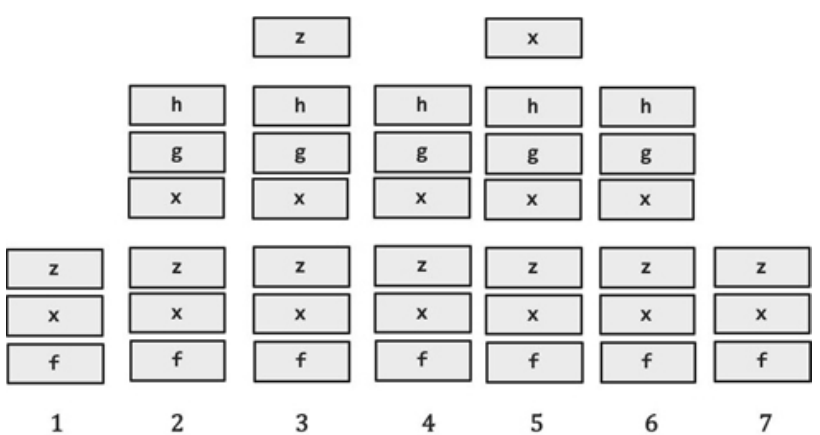
\includegraphics[width=0.8\textwidth]{pics/stack_frame.png}
            \caption{Stack Frame}
        \end{figure}
    \end{frame}

\begin{frame}[fragile]
\frametitle{Common Issue: Not Defined}
\begin{lstlisting}[language=Python]
def f(x):
    def g():
        print(x)
g()
\end{lstlisting}
\end{frame}

    % Stack Frames & Closures Explanation
\begin{frame}{Understanding Stack Frames \& Closures in Python}
    \begin{itemize}
        \item When a function returns, its \textbf{stack frame} is destroyed.
        \item However, Python functions are \textbf{first-class objects} and can be returned.
        \item \textbf{Closures} allow a function to retain access to variables from its enclosing scope.
        \item This is why a function returned from another function can still access variables from the outer function.
    \end{itemize}
\end{frame}


\begin{frame}[fragile]
    \frametitle{Common Issue: UnboundLocalError}
    \begin{lstlisting}[language=Python]
    def f():
        print(x)
    def g():
        print(x)
        x = 1
    x = 3
    f()
    x = 3
    g()
    \end{lstlisting}
\end{frame}
% UnboundLocalError Explanation
\begin{frame}[fragile]
    \frametitle{Common Issue: UnboundLocalError}
    \begin{lstlisting}[language=Python]
def f(x):
    def g():
        x = x + 1  # This will cause an UnboundLocalError
        print("x =", x)
    return g
x = 3
z = f(x)
z()  # Causes an error
    \end{lstlisting}
    \textbf{Why does this happen?}
    \begin{itemize}
        \item Python assumes `x` inside `g` is a new local variable.
        \item Since `x` is used before being assigned, it raises an error.
    \end{itemize}
\end{frame}


% Fixing the Issue with Nonlocal
\begin{frame}[fragile]
    \frametitle{Fix: Using `nonlocal`}
    \begin{lstlisting}[language=Python]
def f(x):
    def g():
        nonlocal x  # Tell Python to use x from f's scope
        x = x + 1
        print("x =", x)
    return g
x = 3
z = f(x)
z()  # Works correctly
    \end{lstlisting}
    \textbf{Key Fix:}
    \begin{itemize}
        \item `nonlocal x` tells Python to modify `x` from `f` instead of creating a new local variable.
    \end{itemize}
\end{frame}


  \begin{frame}{The \texttt{nonlocal} Keyword}
    \begin{itemize}
      \item Used to modify variables in the nearest enclosing (non-global) scope.
      \item Allows inner functions to change variables from outer functions.
      \item Prevents creation of new local variables with the same name.
    \end{itemize}
  \end{frame}

  \begin{frame}[fragile]
    \frametitle{Counter Example}
    \begin{lstlisting}[language=Python]
    def counter():
        count = 0
        def increment():
            nonlocal count
            count += 1
            return count
        return increment
    c = counter()
    print(c())
    print(c())
    print(c())
    \end{lstlisting}
  \end{frame}